\section{Results}
\label{sec:results}

\subsection{First-Order RC Response}
\label{ssec:rc_results}

For the RC sub-circuit, the governing equation can be written as
\begin{equation}
  \dot{\vC} = \frac{\Vs - \vC}{RC}.
  \label{eq:rc_phase}
\end{equation}
The equilibrium is $\vC^\ast=\Vs=\qty{10}{\volt}$.
If $\vC<\Vs$, then $\dot{\vC}>0$; if $\vC>\Vs$, then $\dot{\vC}<0$.
Thus the phase line points toward $\vC^\ast$ from both sides, so the
equilibrium is asymptotically stable.

Using $R=\qty{100}{\ohm}$ and $C=\qty{10}{\micro\farad}$ gives
$\tau_{RC}=RC=\qty{1}{\milli\second}$.
For three initial capacitor voltages,
\begin{align}
  \vC(t;V_0=0) &= 10\left(1-e^{-1000t}\right), \label{eq:rc_v0_0}\\
  \vC(t;V_0=5) &= 10 - 5e^{-1000t}, \label{eq:rc_v0_5}\\
  \vC(t;V_0=10) &= 10. \label{eq:rc_v0_10}
\end{align}
All three cases approach the same stable equilibrium, but they start from
different points on the phase line.

With $V_0=0$ fixed and $C=\qty{10}{\micro\farad}$, varying resistance changes
only the time constant:
\begin{align}
  R=\qty{50}{\ohm}: \quad \vC(t) &= 10\left(1-e^{-2000t}\right),
    \label{eq:rc_r_50}\\
  R=\qty{100}{\ohm}: \quad \vC(t) &= 10\left(1-e^{-1000t}\right),
    \label{eq:rc_r_100}\\
  R=\qty{200}{\ohm}: \quad \vC(t) &= 10\left(1-e^{-500t}\right).
    \label{eq:rc_r_200}
\end{align}
Larger resistance produces slower charging, which is the first-order analog
of the damping effect studied in the full RLC circuit.

\subsection{Second-Order RLC Response}
\label{ssec:rlc_results}

For the selected component values,
\begin{equation}
  \omega_0 = \qty{1000}{\radian\per\second}, \qquad
  \Rcrit = \qty{200}{\ohm}.
  \label{eq:numerical_omega_rcrit}
\end{equation}
The three resistance values in Table~\ref{tab:damping-cases} therefore
sample the underdamped, critically damped, and overdamped regimes without
changing $L$, $C$, or the source voltage.

\begin{table}[!t]
  \caption{Damping Cases for the Series RLC Step Response}
  \label{tab:damping-cases}
  \centering
  \begin{tabular}{@{}llll@{}}
    \toprule
    Case & $R$ & $\alpha$ & Characteristic data \\
    \midrule
    Underdamped & \qty{50}{\ohm} & \qty{250}{\per\second}
      & $\omega_d = \qty{968.25}{\radian\per\second}$ \\
    Critically damped & \qty{200}{\ohm} & \qty{1000}{\per\second}
      & $r = \qty{-1000}{\per\second}$ \\
    Overdamped & \qty{500}{\ohm} & \qty{2500}{\per\second}
      & $r_1 = \qty{-208.71}{\per\second}$,
        $r_2 = \qty{-4791.29}{\per\second}$ \\
    \bottomrule
  \end{tabular}
\end{table}

With $\vC(0)=0$, $\dot{\vC}(0)=0$, and $\Vs=\qty{10}{\volt}$, the numerical
step responses are as follows, with $t$ measured in seconds and $\vC$ measured
in volts:
\begin{align}
  v_{C,50}(t)
    &= 10\!\left[
      1 - e^{-250t}\!\left(\cos(968.25t)
      + 0.2582\sin(968.25t)\right)\right],
      \label{eq:under_numeric}\\
  v_{C,200}(t)
    &= 10\!\left[1 - (1 + 1000t)e^{-1000t}\right],
      \label{eq:crit_numeric}\\
  v_{C,500}(t)
    &= 10 - 10.456e^{-208.71t} + 0.456e^{-4791.29t}.
      \label{eq:over_numeric}
\end{align}
Equation~\eqref{eq:under_numeric} oscillates around the final value before
settling, \eqref{eq:crit_numeric} reaches the final value as quickly as
possible without oscillation, and \eqref{eq:over_numeric} approaches the
final value without overshoot but is slowed by the dominant pole
$r_1 = \qty{-208.71}{\per\second}$.

\begin{figure}[htbp]
  \centering
  \begin{tikzpicture}
    \begin{axis}[
      width=0.92\columnwidth,
      height=6cm,
      grid=both,
      xmin=0, xmax=0.03,
      ymin=0, ymax=18,
      xlabel={$t$ (\si{\second})},
      ylabel={$\vC(t)$ (\si{\volt})},
      legend pos=south east,
      legend cell align=left
    ]
      \addplot[blue, thick, samples=450, domain=0:0.03]
        {10*(1 - exp(-250*x)*(cos(deg(968.25*x)) + 0.2582*sin(deg(968.25*x))))};
      \addlegendentry{$R=\qty{50}{\ohm}$}
      \addplot[red!70!black, thick, dashed, samples=300, domain=0:0.03]
        {10*(1 - (1 + 1000*x)*exp(-1000*x))};
      \addlegendentry{$R=\qty{200}{\ohm}$}
      \addplot[green!50!black, thick, dash dot, samples=300, domain=0:0.03]
        {10 - 10.456*exp(-208.71*x) + 0.456*exp(-4791.29*x)};
      \addlegendentry{$R=\qty{500}{\ohm}$}
      \addplot[black!55, thin, dotted, domain=0:0.03] {10};
      \addlegendentry{Final value}
    \end{axis}
  \end{tikzpicture}
  \caption{Capacitor voltage $\vC(t)$ for three values of resistance $R$,
           showing underdamped, critically damped, and overdamped responses.}
  \label{fig:vc_vs_t}
\end{figure}

\begin{figure}[htbp]
  \centering
  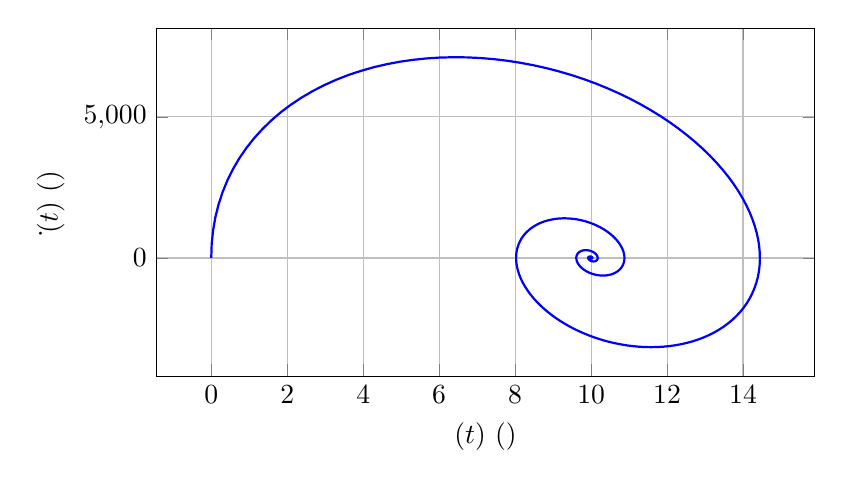
\begin{tikzpicture}
    \begin{axis}[
      width=0.82\columnwidth,
      height=6cm,
      grid=both,
      xlabel={$\vC(t)$ (\si{\volt})},
      ylabel={$\dot{\vC}(t)$ (\si{\volt\per\second})}
    ]
      \addplot[blue, thick, samples=600, domain=0:0.03]
        ({10*(1 - exp(-250*x)*(cos(deg(968.25*x)) + 0.2582*sin(deg(968.25*x))))},
         {10*exp(-250*x)*(1000000/968.25)*sin(deg(968.25*x))});
    \end{axis}
  \end{tikzpicture}
  \caption{Phase portrait of the second-order system ($\dot{\vC}$ vs.\ $\vC$)
           for the underdamped case with $R = \qty{50}{\ohm}$.}
  \label{fig:phase}
\end{figure}

\subsection{Connection to the Research Question}

The results show that changing $R$ changes the characteristic roots while
leaving the energy-storage parameters $L$ and $C$ fixed. For
$R=\qty{50}{\ohm}$, the roots are complex and the capacitor voltage rings
before settling. For $R=\qty{200}{\ohm}$, the repeated real root gives the
fastest non-oscillatory response. For $R=\qty{500}{\ohm}$, two negative real
roots remove oscillation but slow the return to equilibrium. Thus resistance
directly controls the damping mechanism described in the research question.
